\documentclass[aspectratio=169]{beamer}
\usepackage{babel}
\usepackage{array, colortbl, tikz, transparent, listings, pgfplots}
\usepackage[export]{adjustbox}
\usepackage[skins,theorems]{tcolorbox}
\usepackage[backend=biber,style=verbose-ibid,citetracker=true,ibidtracker=constrict,autocite=footnote]{biblatex}

\setbeamercovered{transparent}
\lstdefinelanguage{Rust}{
    sensitive=true,
    morekeywords={as, break, const, continue, crate, else, enum, extern, false, fn, for, if, impl, in, let, loop, match, mod, move, mut, pub, ref, return, self, Self, static, struct, super, trait, true, type, unsafe, use, where, while, async, await, dyn, Result, Option, Ok, Err, panic},
    morecomment=[l]{//},
    morecomment=[s]{/*}{*/},
    morestring=[b]",
    morestring=[b]',
}
\lstdefinelanguage{Yaml}{
    sensitive=true,
    morekeywords={true, false, null, particles, type, cuboid, foreach, position, velocity, mass, sigma, brownian_sigma},
    morecomment=[l]{\#},
    morestring=[b]",
}
\lstset{
    language=Rust,
    basicstyle=\ttfamily\small,
    keywordstyle=\color{blue}\bfseries,
    stringstyle=\color{red},
    commentstyle=\color{teal},
    morekeywords={Result, Option, Ok, Err, Some, None, panic},
    breaklines=true
}
\usetikzlibrary{automata,positioning}
\addbibresource{Reference.bib}

\title{Rust vs C++: Brief Introduction}
\author{Anatoly Weinstein}
\date{30th of April 2025}

\newcommand{\framebackground}[3]{
    \begin{tikzpicture}
        \transparent{#1}
        \node[inner sep=0] at (current page.center) {
            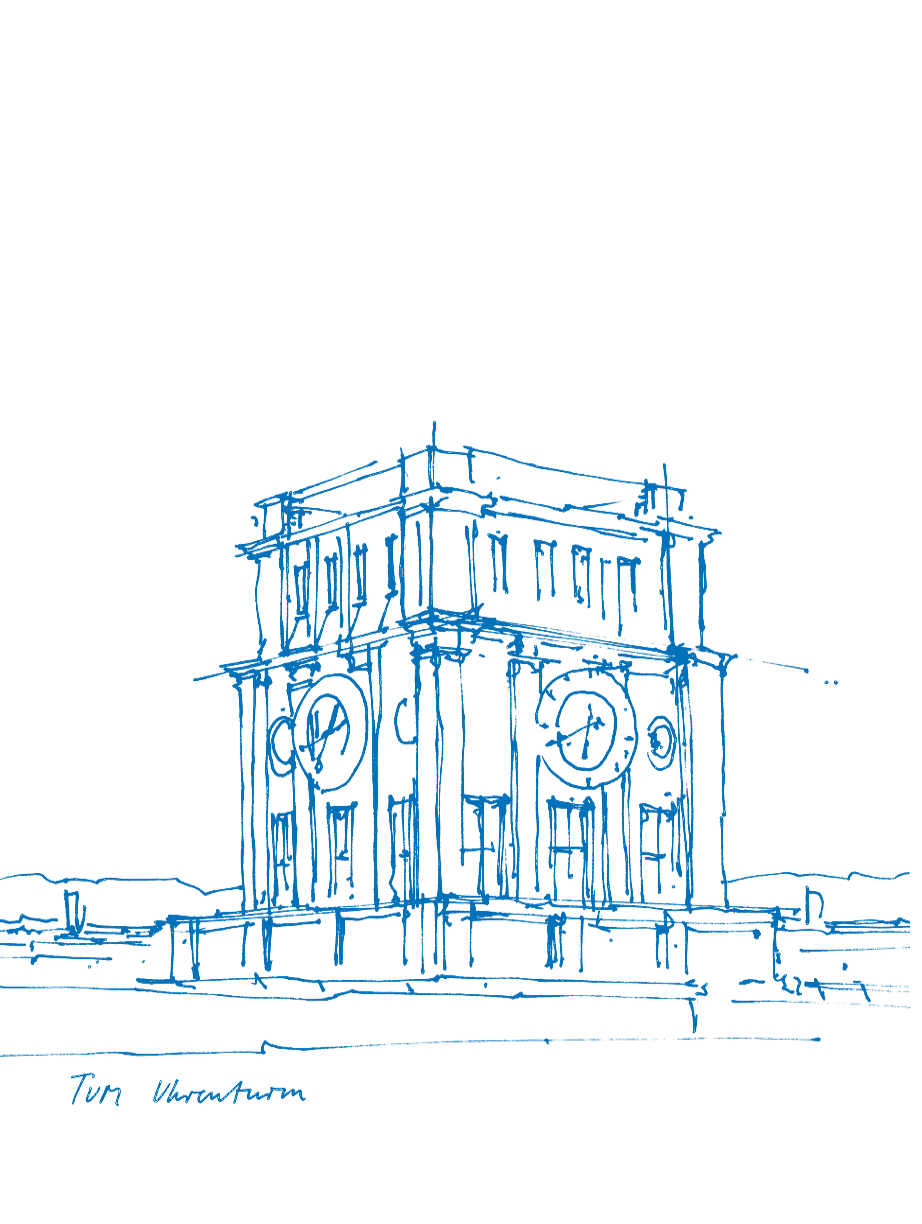
\includegraphics[height=\paperheight, right]{./media/tum-uhrenturm.png}
        };
        \transparent{#2}
        \node[anchor=south, text width=\paperwidth, text height=1.5cm, draw=none, align=center] at (current page.south) {
            \insertpagenumber
        };
        \transparent{#3}
        \node[anchor=south, text width=\paperwidth, text height=1.5cm, draw=none, align=right] at (current page.south) {
            \small Anatoly W. \,\,
        };
    \end{tikzpicture}
}

\newcommand{\headerframe}{
    \usebackgroundtemplate{
        \framebackground{0.2}{1}{1}
    }
}

\newcommand{\simpleframe}{
    \usebackgroundtemplate{
        \framebackground{0}{1}{1}
    }
}

\newcommand{\nofooterframe}{
    \usebackgroundtemplate{
        \framebackground{0}{0}{1}
    }
}

\newcommand{\blue}[1]{{\color{beamer@blendedblue} #1}}
\newcommand{\yellow}[1]{{\color[HTML]{AF8F10} #1}}
\newcommand{\gray}[1]{{\color[HTML]{8F8F8F} #1}}
\newcommand{\red}[1]{{\color[HTML]{FF5F5F} #1}}

\begin{document}

%
% Frame
%
\usebackgroundtemplate{\framebackground{0.2}{0}{0}}
\begin{frame}
    \maketitle
\end{frame}

\nofooterframe\begin{frame}{Cross-Language Benchmark Results\footcite{benchmark-1}\footcite{benchmark-15}}
    \begin{center}
        \begin{tikzpicture}
            \begin{axis}[
                width=\textwidth,  
                height=0.7\textheight,
                xlabel={},
                ylabel={Runtime (ms)},
                xtick={0, 20, 50},
                scaled x ticks=false,  
                scaled y ticks=false,
                ymajorgrids=true, 
                grid style=dashed,
                xmin=-5,
                xmax=55,
                legend style={at={(0.05,0.95)},anchor=north west},
            ]

            \addplot[
                color=blue,
                mark=square,
                line width=1pt,
                ]
                coordinates {
                    (0, 109)(20, 509)(50, 1080)
                };

            \addplot[
                color=orange,
                mark=triangle,
                line width=1pt,
                ]
                coordinates {
                    (0, 66)(20, 1046)(50, 2522)
                };

            \addplot[
                color=cyan,
                mark=square,
                line width=1pt,
                ]
                coordinates {
                    (20, 454)(50, 1031)
                };

            \addplot[
                color=red,
                mark=triangle,
                line width=1pt,
                ]
                coordinates {
                    (20, 979)(50, 2478)
                };

            \legend{C++ (Ci 11), Rust (Ci 11), C++ (Ci 15), Rust (Ci 15)}
            \end{axis}
        \end{tikzpicture}
    \end{center}

    \vspace{-0.2em}
    The workflow 15 removed printing output and records average of 5 runs.
\end{frame}

\nofooterframe\begin{frame}{Cross-Algorithm Benchmark Results\footcite{benchmark-1}\footcite{benchmark-22}}
    \begin{center}
        \begin{tikzpicture}
            \begin{axis}[
                width=\textwidth,  
                height=0.7\textheight,
                xlabel={},
                ylabel={Runtime (ms)},
                xtick={0, 20, 50},
                scaled x ticks=false,  
                scaled y ticks=false,
                ymajorgrids=true, 
                grid style=dashed,
                xmin=-5,
                xmax=55,
                legend style={at={(0.05,0.95)},anchor=north west},
            ]

            \addplot[
                color=blue,
                mark=square,
                line width=1pt,
                ]
                coordinates {
                    (0, 109)(20, 509)(50, 1080)
                };

            \addplot[
                color=orange,
                mark=triangle,
                line width=1pt,
                ]
                coordinates {
                    (0, 66)(20, 1046)(50, 2522)
                };

            \addplot[
                color=cyan,
                mark=square,
                line width=1pt,
                ]
                coordinates {
                    (20, 83)(50, 178)
                };

            \addplot[
                color=red,
                mark=triangle,
                line width=1pt,
                ]
                coordinates {
                    (20, 589)(50, 1316)
                };

            \legend{C++ (direct-sum), Rust (direct-sum), C++ (linked-cells), Rust (linked-cells)}
            \end{axis}
        \end{tikzpicture}
    \end{center}

    The cell size has been set to 5.0 units in every dimension for both implementations. \blue{Current C++ \texttt{direct-sum} implementation outperforms Rust \texttt{linked-cells}} on the \texttt{two-bodies-collision} input.
\end{frame}

\nofooterframe\begin{frame}[t,fragile]{Performance Tool: \texttt{perf}}
    Linux only.

    \begin{lstlisting}
echo 0 | sudo tee /proc/sys/kernel/perf_event_paranoid
    \end{lstlisting}

    First we fix missing permissions.\footcite{perf-fix-permissions}

    \begin{lstlisting}
perf record <command>
    \end{lstlisting}

    This will run the command and record performance by taking snapshots of the stack. This requires projects to be built in \blue{release mode} but with \blue{debug symbols}. This will write everything to the file \texttt{perf.data}.\ \gray{Apparently we don't need this for Rust.}

    In our case, \texttt{<command>} is roughly equivalent to the call \texttt{./target/.../moldyn input/... -s 0 -t ...}

    When the file was created, we can analyze it with:

    \begin{lstlisting}
perf report
    \end{lstlisting}
\end{frame}

\nofooterframe\begin{frame}[t]{Performance Hotspots: C++ vs Rust (Direct Sum)}
    \centering
    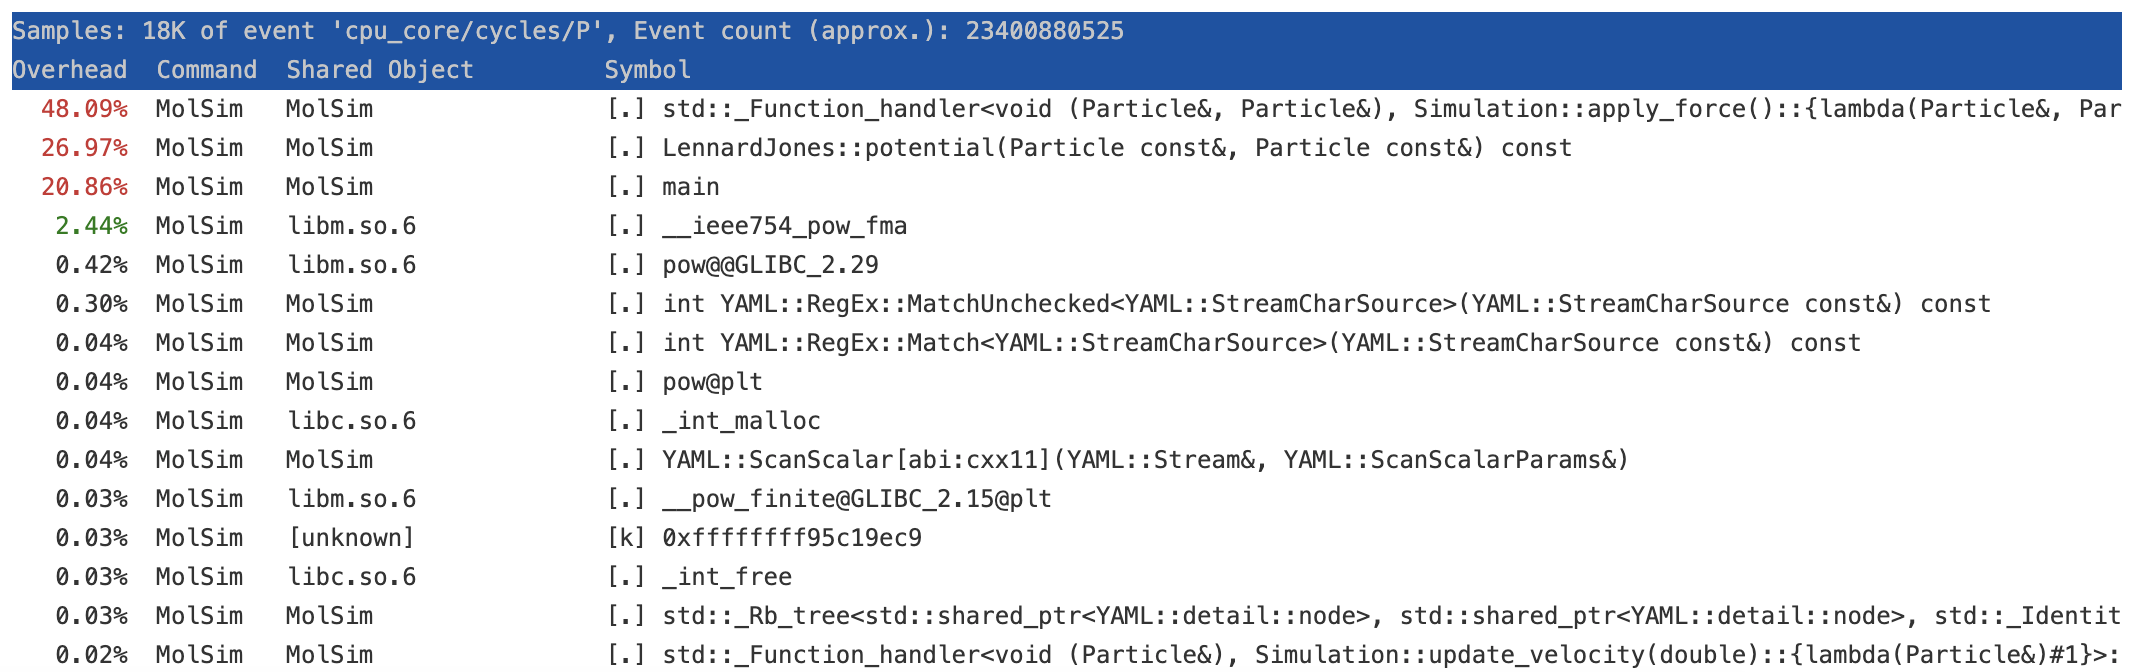
\includegraphics[width=0.8\textwidth]{media/perf-cpp-1-directsum.png}
    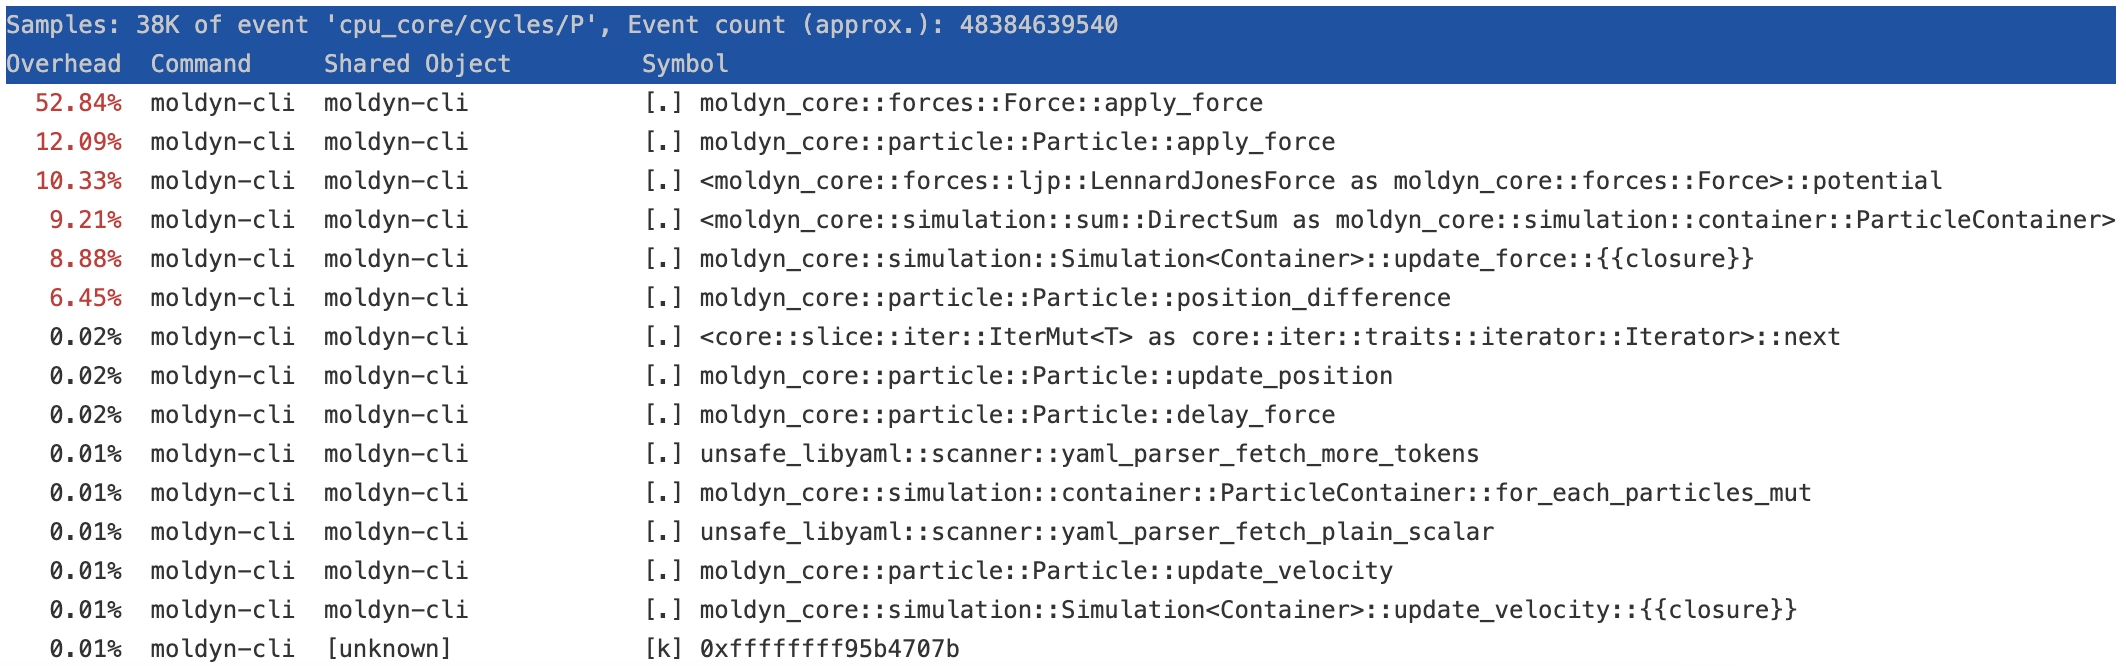
\includegraphics[width=0.8\textwidth]{media/perf-rs-1-directsum.png}
\end{frame}

\nofooterframe\begin{frame}[t]{Performance Hotspots: C++ vs Rust (Linked Cells)}
    \begin{columns}[T,onlytextwidth]
        \begin{column}{0.5\textwidth}
            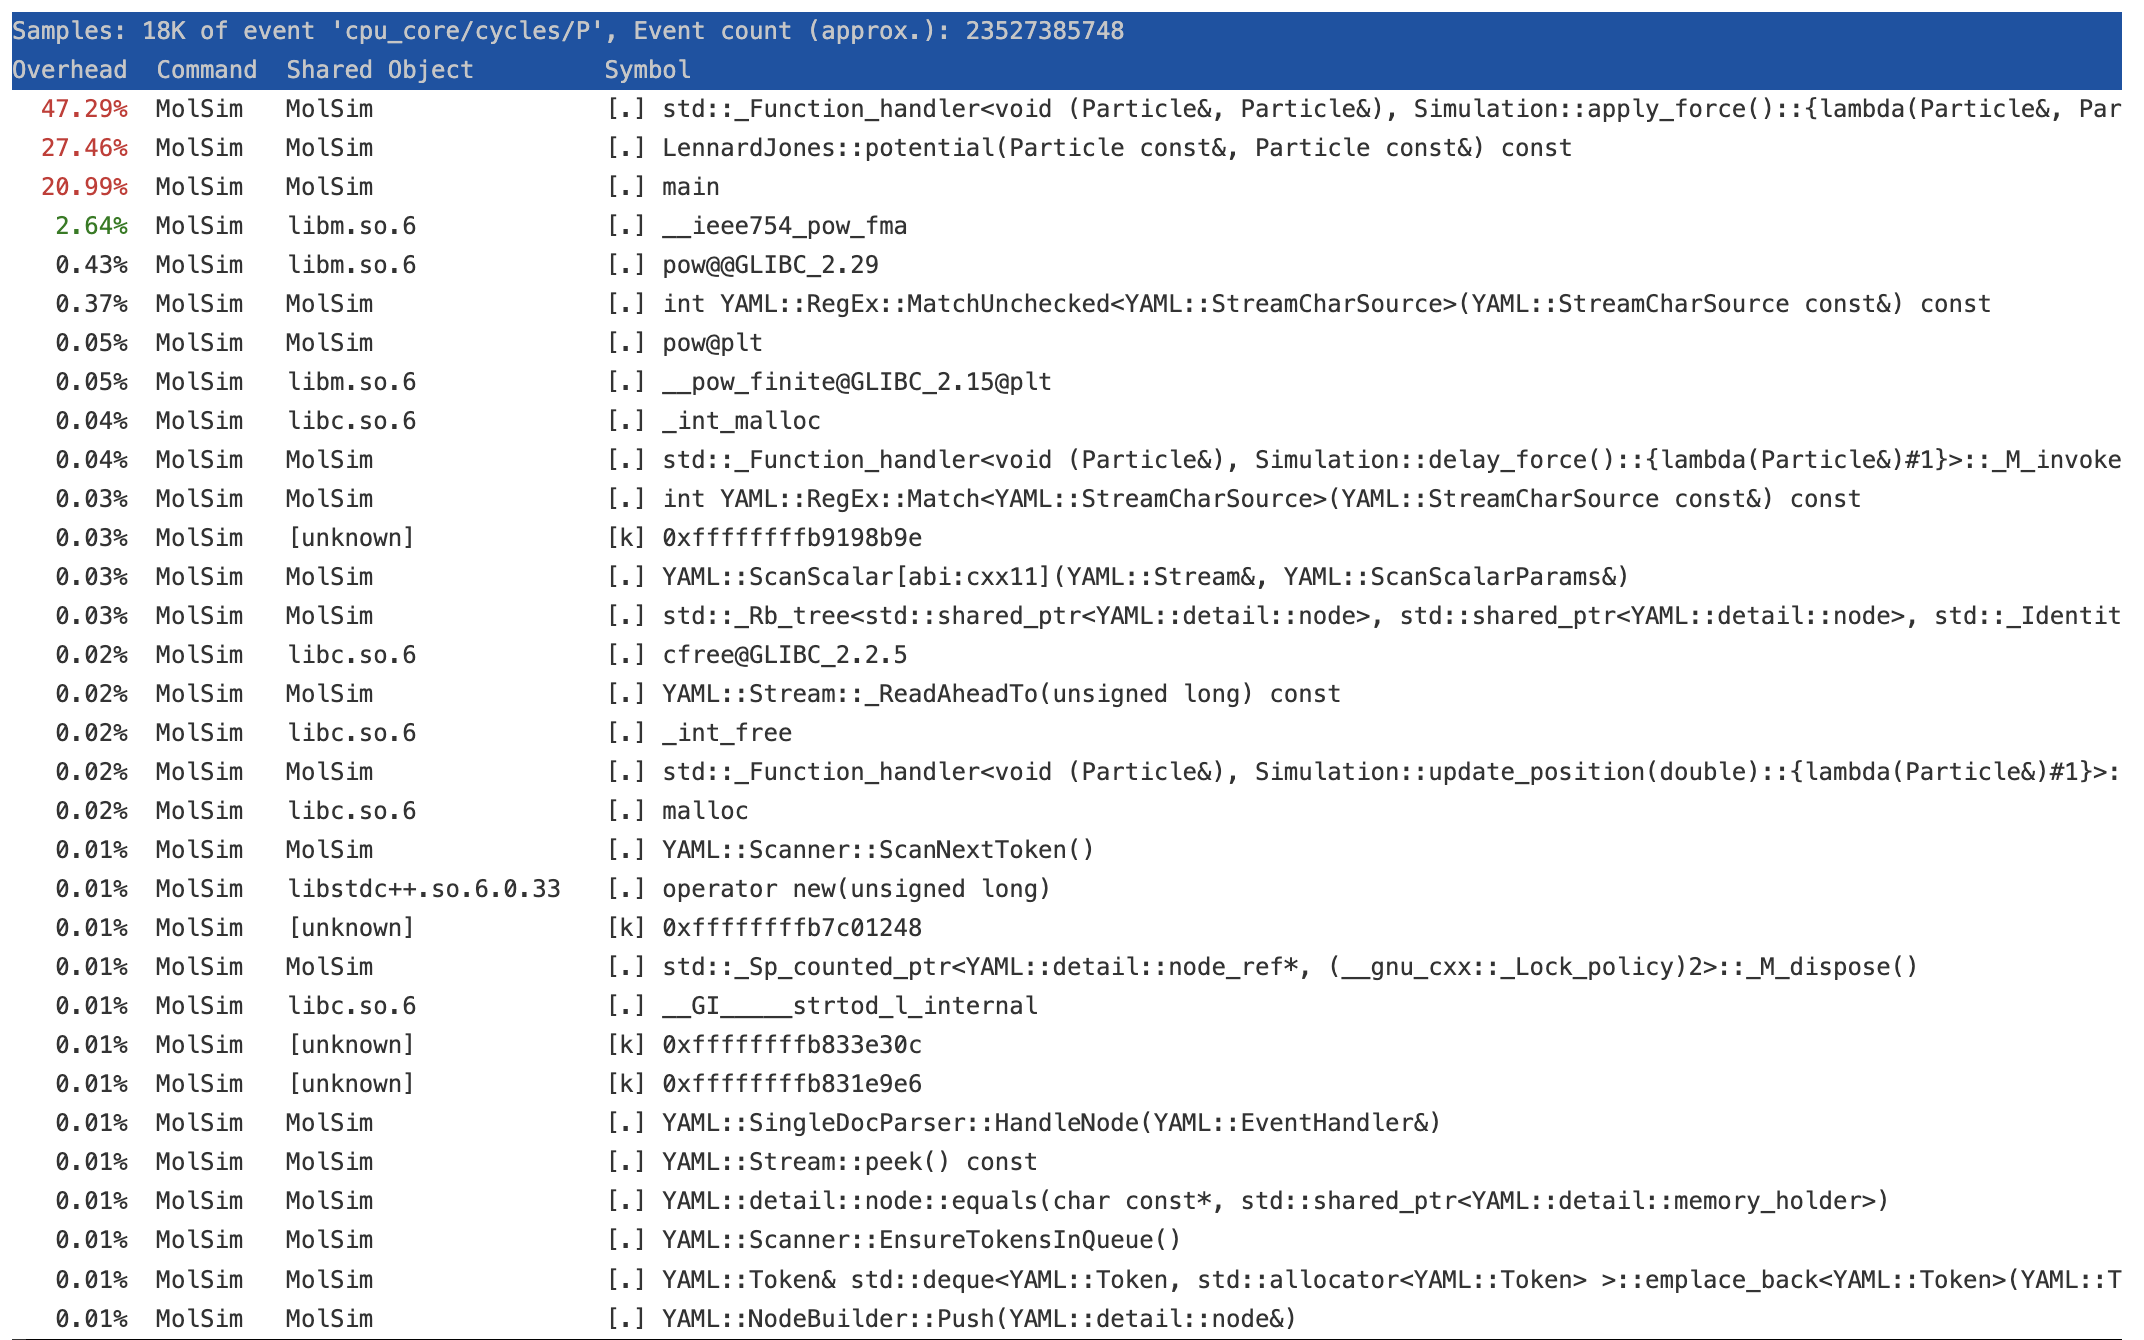
\includegraphics[width=\textwidth]{media/perf-cpp-1.png}
        \end{column}
        \begin{column}{0.5\textwidth}
            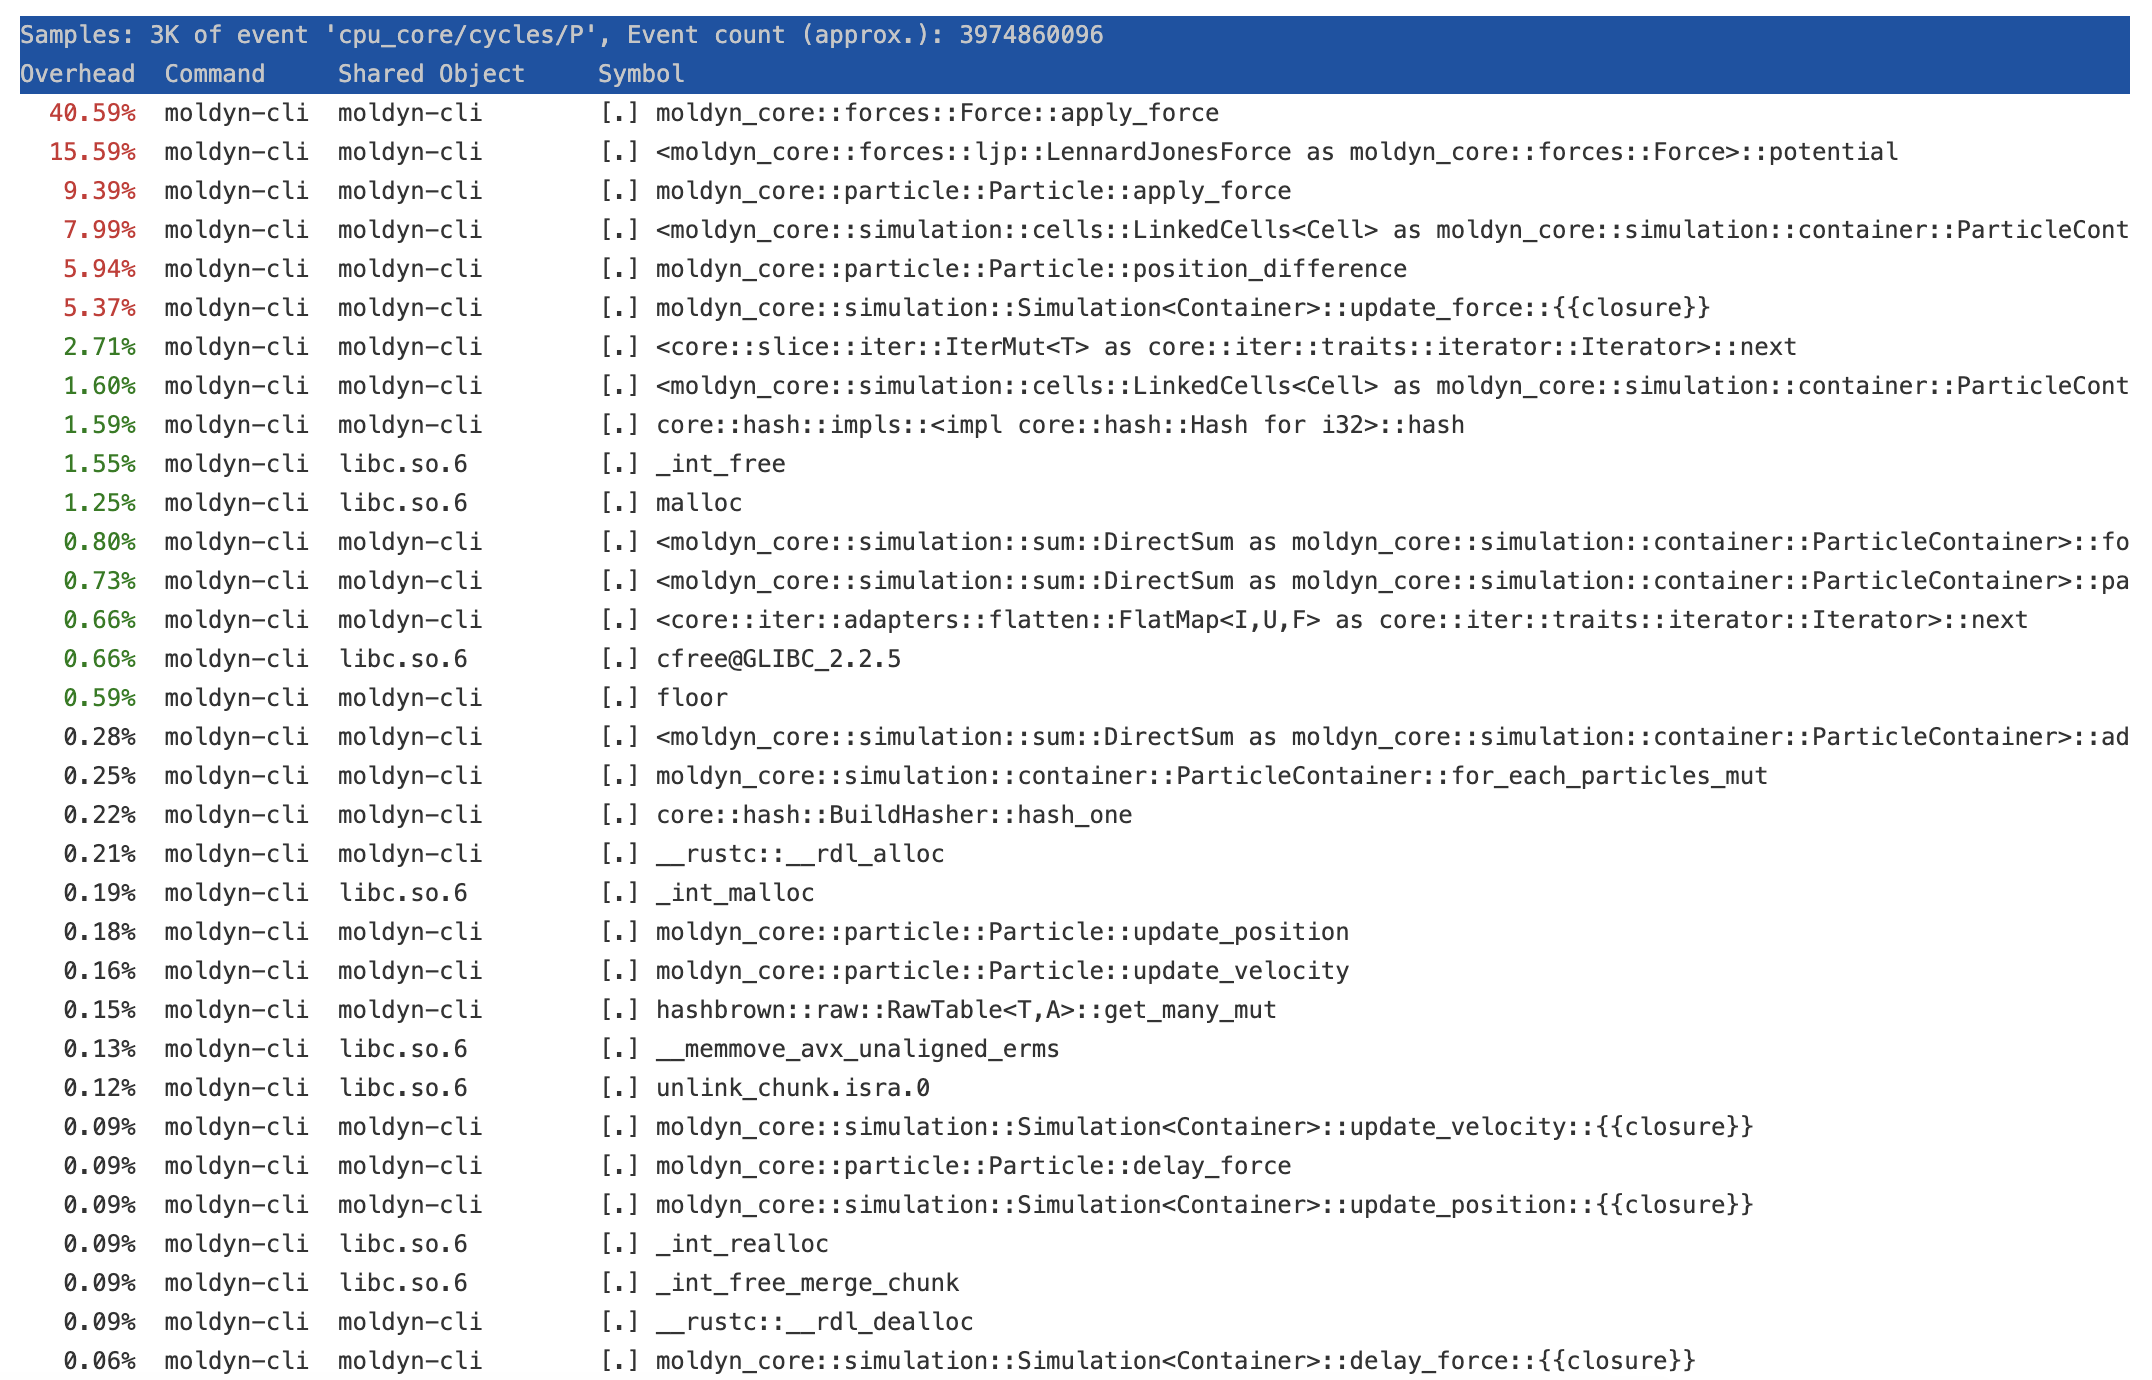
\includegraphics[width=\textwidth]{media/perf-rs-1.png}
        \end{column}
    \end{columns}
\end{frame}

\nofooterframe\begin{frame}[t]{Performance Hotspots: C++}
    Only three severe hotspots, covering 95\% of the runtime:

    \vspace{0.5em}
    \begin{tabular}{ m{0.16\textwidth} m{0.76\textwidth} } 
        \blue{47.29\%} & Pairwise iteration \\
        \blue{27.46\%} & Lennard Jones Potential \\
        \blue{20.99\%} & Program Frame \\
        2.64\% & Power Function \\
        1.62\% & Other
    \end{tabular}

    % \begin{enumerate}
    %     \item Pairwise iteration
    %     \item Lennard Jones Potential
    %     \item Program Frame
    % \end{enumerate}
\end{frame}

\nofooterframe\begin{frame}[t]{Performance Hotspots: Attempts at Optimization}
    A lot of hotspots, explaining the runtime of the Rust implementation. It seems to be an implementation-problem and not a language-problem.

    I believe, in summary, the \blue{hotspots in the Rust implementation are caused} by the following:

    \begin{enumerate}
        \item \textbf{Codeflow security, overflow checks}, validation of data, etc. (Example: slower but secure \texttt{<Hash for i32>::hash} function hotspot)
        \item Different \blue{memory strategy} for \blue{Rust vectors} and \blue{C++ vectors}, leading to more \blue{allocations and frees}. (Reason: Allocation hotspot in linked cells run.)
        \item Different allocation strategies (\texttt{\_int\_malloc} vs \texttt{malloc})
        \item \blue{Using Iterator abstractions} in Rust, which use inefficient straategies. (Reason: \texttt{<IterMut<T> as Iterator>::next} hotspot)
    \end{enumerate}

    Note: I made a big mistake chosing wrong design patterns in the Rust implementation. (will mention this verbally in the presentation today). Recall: hash implemnentation, iterator implementation.
\end{frame}

\nofooterframe\begin{frame}[t]{Idea for Thesis Table of Contents}
    \begin{enumerate}
        \item Introduction: Companies are switching to Rust, open questions: Why?
        \item Main Contents:
        \begin{enumerate}
            \item Rust Ecosystem: Cargo, Crates (less fragmented)
            \item Syntax Differences, learning curve and the Rust language
            \item Implementation differences and why I used certain 
            \item Benchmarking
        \end{enumerate}
        \item Conclusion: Find evidence where Rust is faster, (data structures?)
    \end{enumerate}
\end{frame}

\headerframe\begin{frame}[allowframebreaks]{References}
  \printbibliography
\end{frame}

\end{document}
